\section{原型系统设计与实现}
本章将根据前文对基于P2P网络的信息自主流动机制的讨论,设计并实现一套较为完善的原型系统。这里系统是指运行在每个节点上既能充当服务器发送信息、也能充当客户端接受信息,我们称之为节点系统。节点系统中作为服务器角色的模块成为节点服务端程序,另外作为客户端角色的模块成为节点客户端程序。本章将分别从节点系统需求分析、架构、数据库、功能模块等方面入手,详细讨论各个实现环节的细节,最后将简单展示节点客户端程序的一些功能。

\subsection{节点系统的总体需求设计}
在本节中,将分析节点系统中各大服务模块的功能,包括节点客户端程序的资源管理功能,以及节点服务器程序中包含的四大功能模块。

\subsubsection{节点客户端程序的需求设计}
\begin{figure}[!ht]
\centering
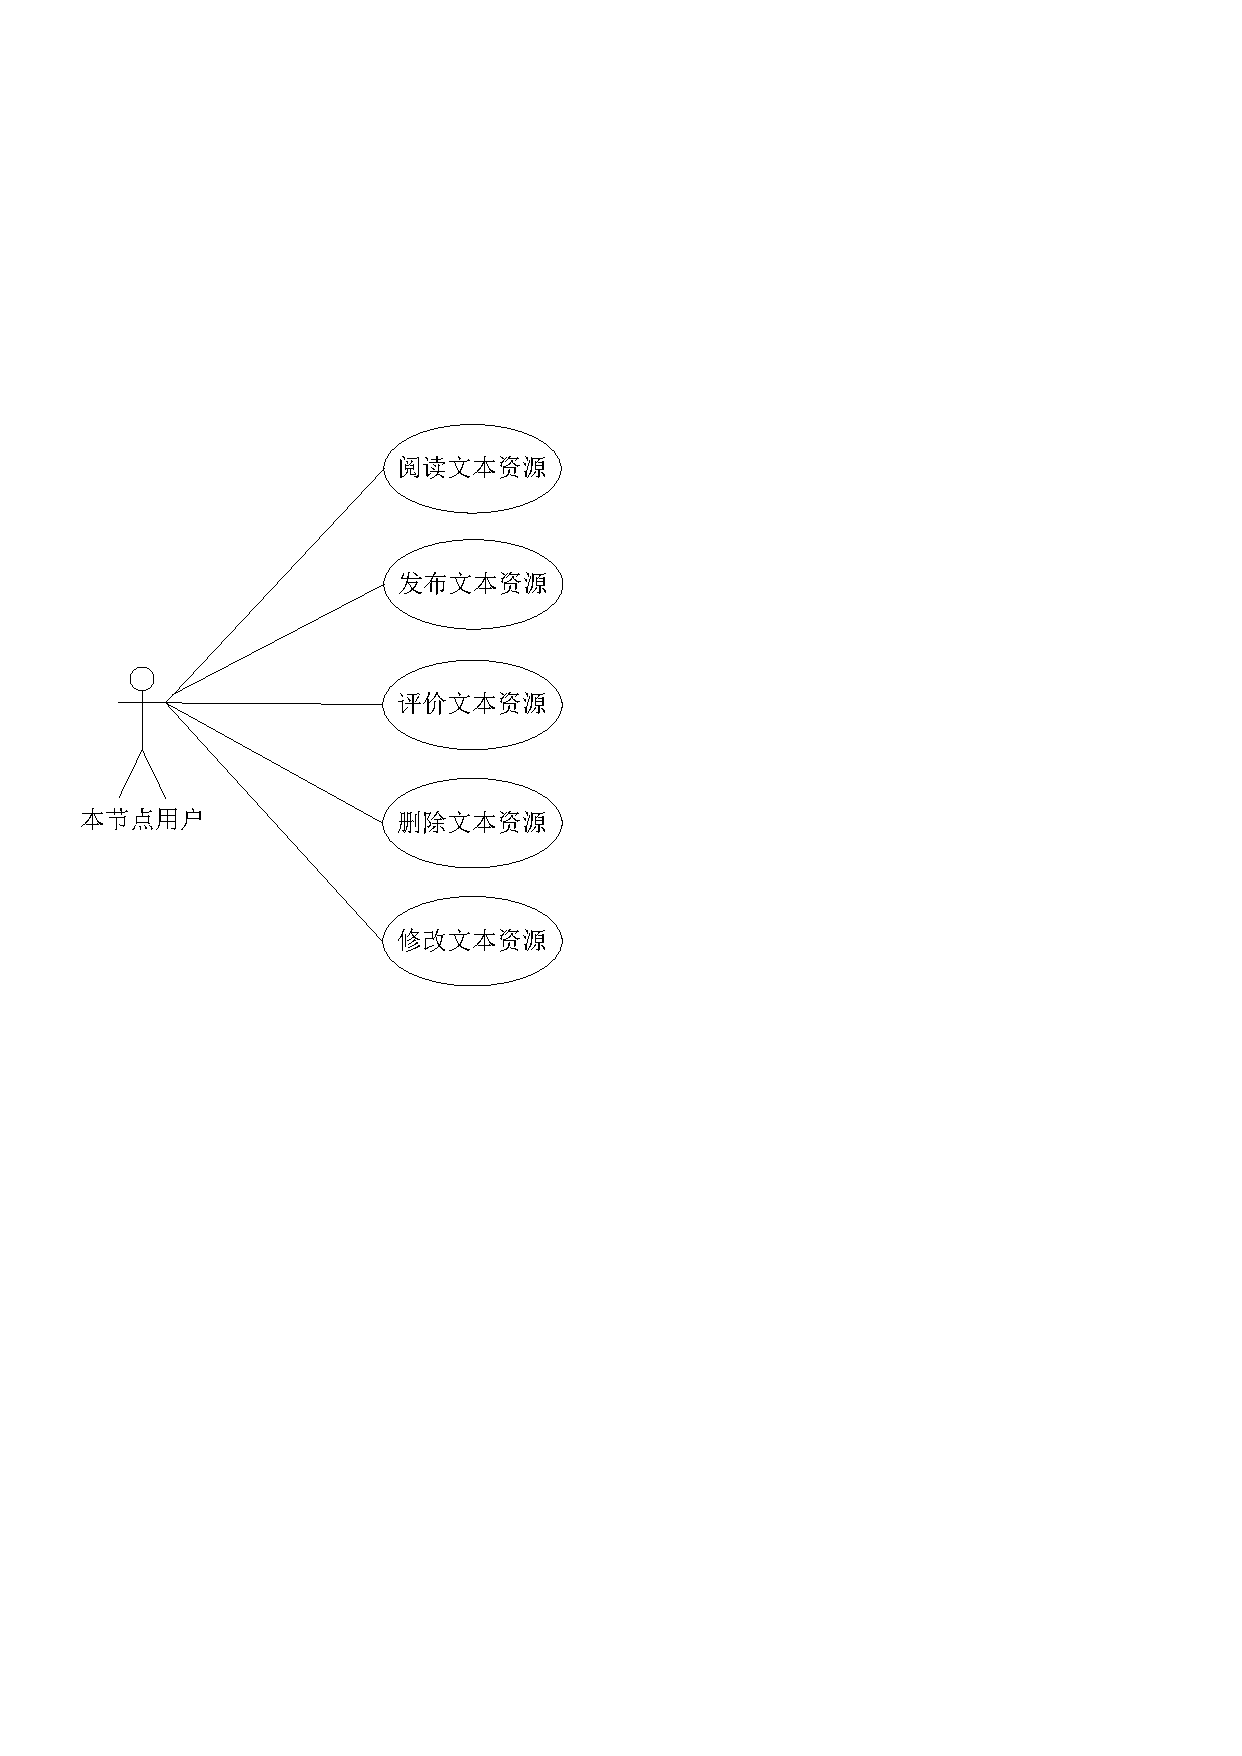
\includegraphics[width=0.6\textwidth]{usecase1.pdf}
\caption{节点客户端程序的用例图}
\label{fig:usecase1}
\end{figure}

该模块的功能比较简单,主要针对的角色是本节点用户,具体的操作包括对文本资源的阅读、删除和修改,以及发布新的文本资源,或对文本资源进行评价和反馈。如图\ref{fig:usercase1}所示,展示了节点客户端程序的用例图。

\subsubsection{服务端资源管理的需求设计}
\begin{figure}[!ht]
\centering
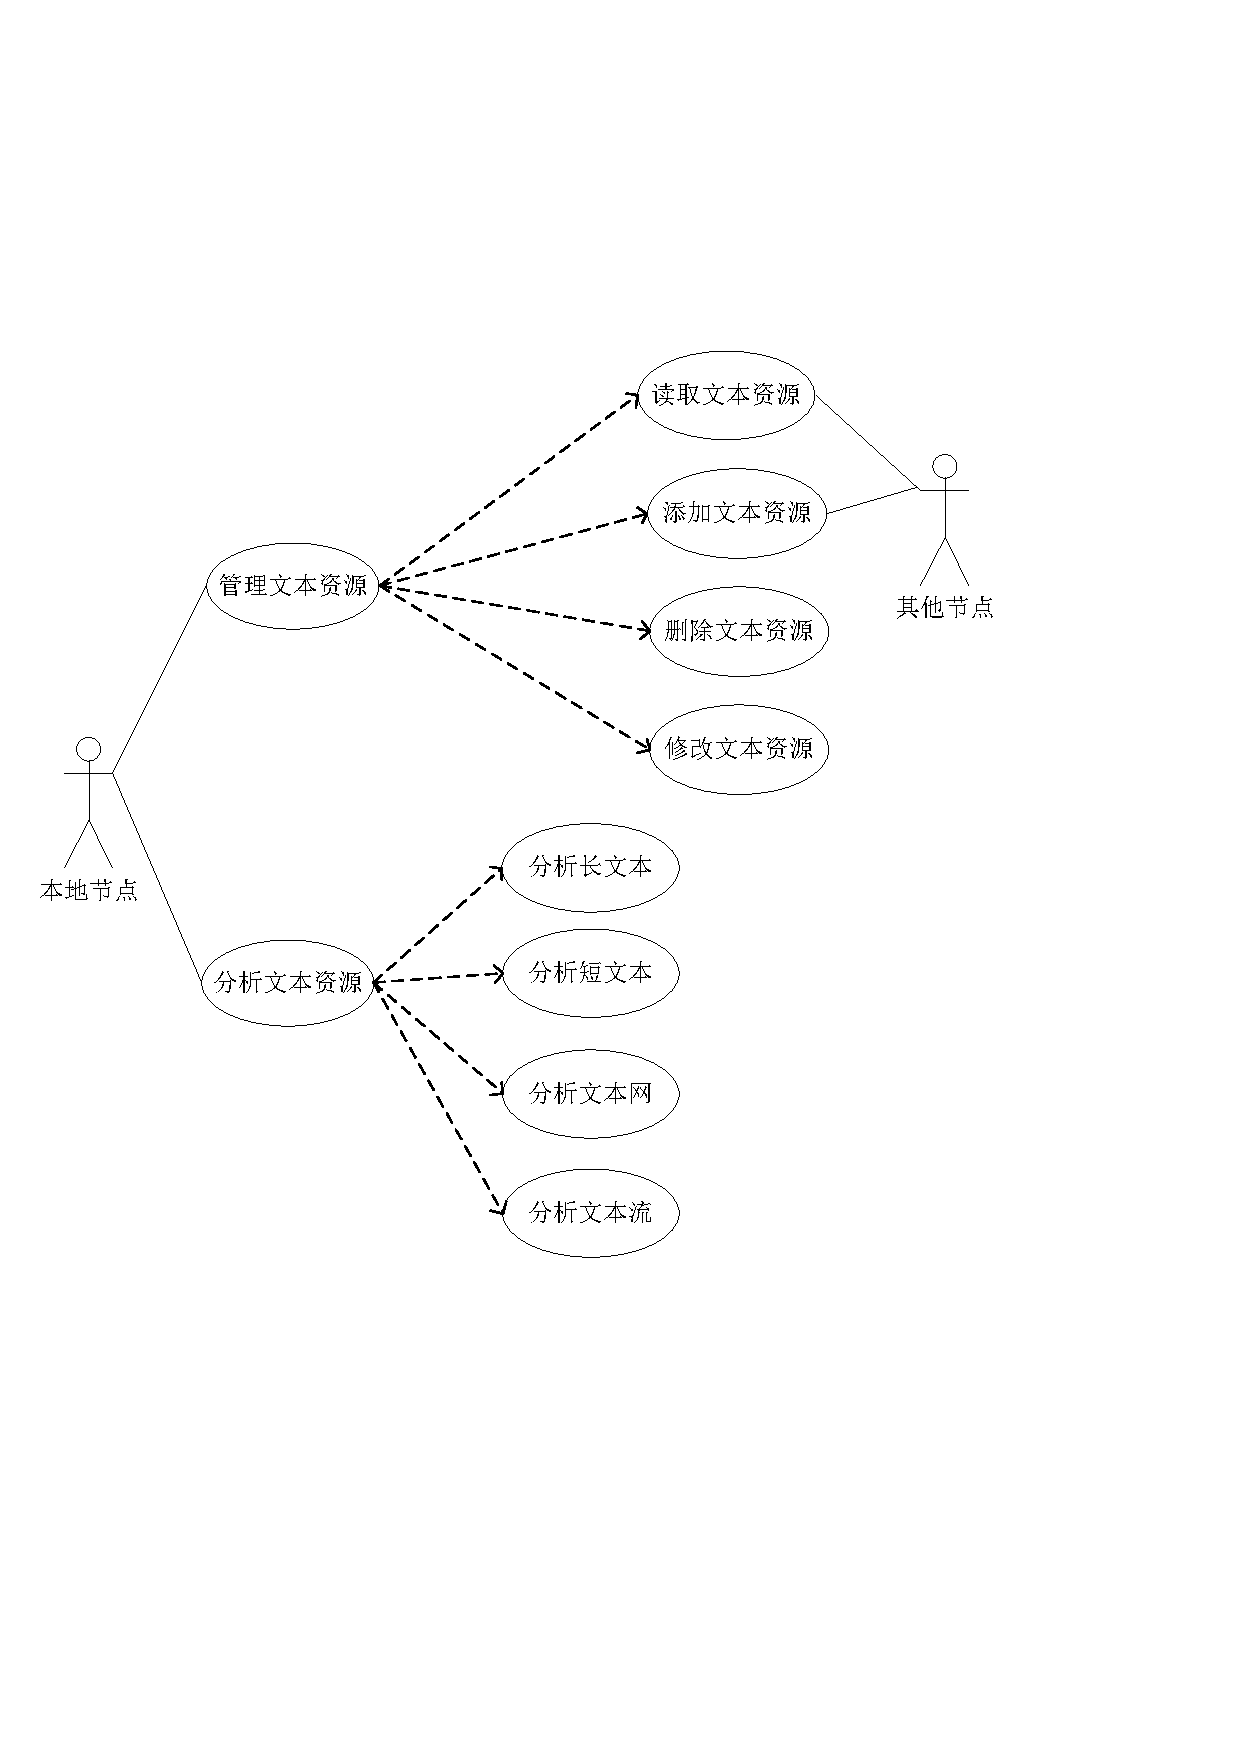
\includegraphics[width=\textwidth]{usecase2.pdf}
\caption{服务端资源管理的用例图}
\label{fig:usecase2}
\end{figure}

该模块的功能主要是对文本资源的进行管理和分析,本地节点拥有所有的功能权限。在管理文本资源模块中,可以对文本资源进行读取、添加、删除和修改的操作。而其他节点只能对文本资源进行读取和添加。在分析文本资源模块中,本地节点可以对四种类型的文本进行分析,包括长文本资源、短文本资源、文本网资源和文本流资源。这四种文本的分析主要是从这些类型的文本中识别出主题,从而在以后的用户兴趣分析中起到作用。如图\ref{fig:usercase2}所示,展示了节点服务端程序中资源管理模块的用例图。

\subsubsection{服务端节点管理的需求设计}
\begin{figure}[!ht]
\centering
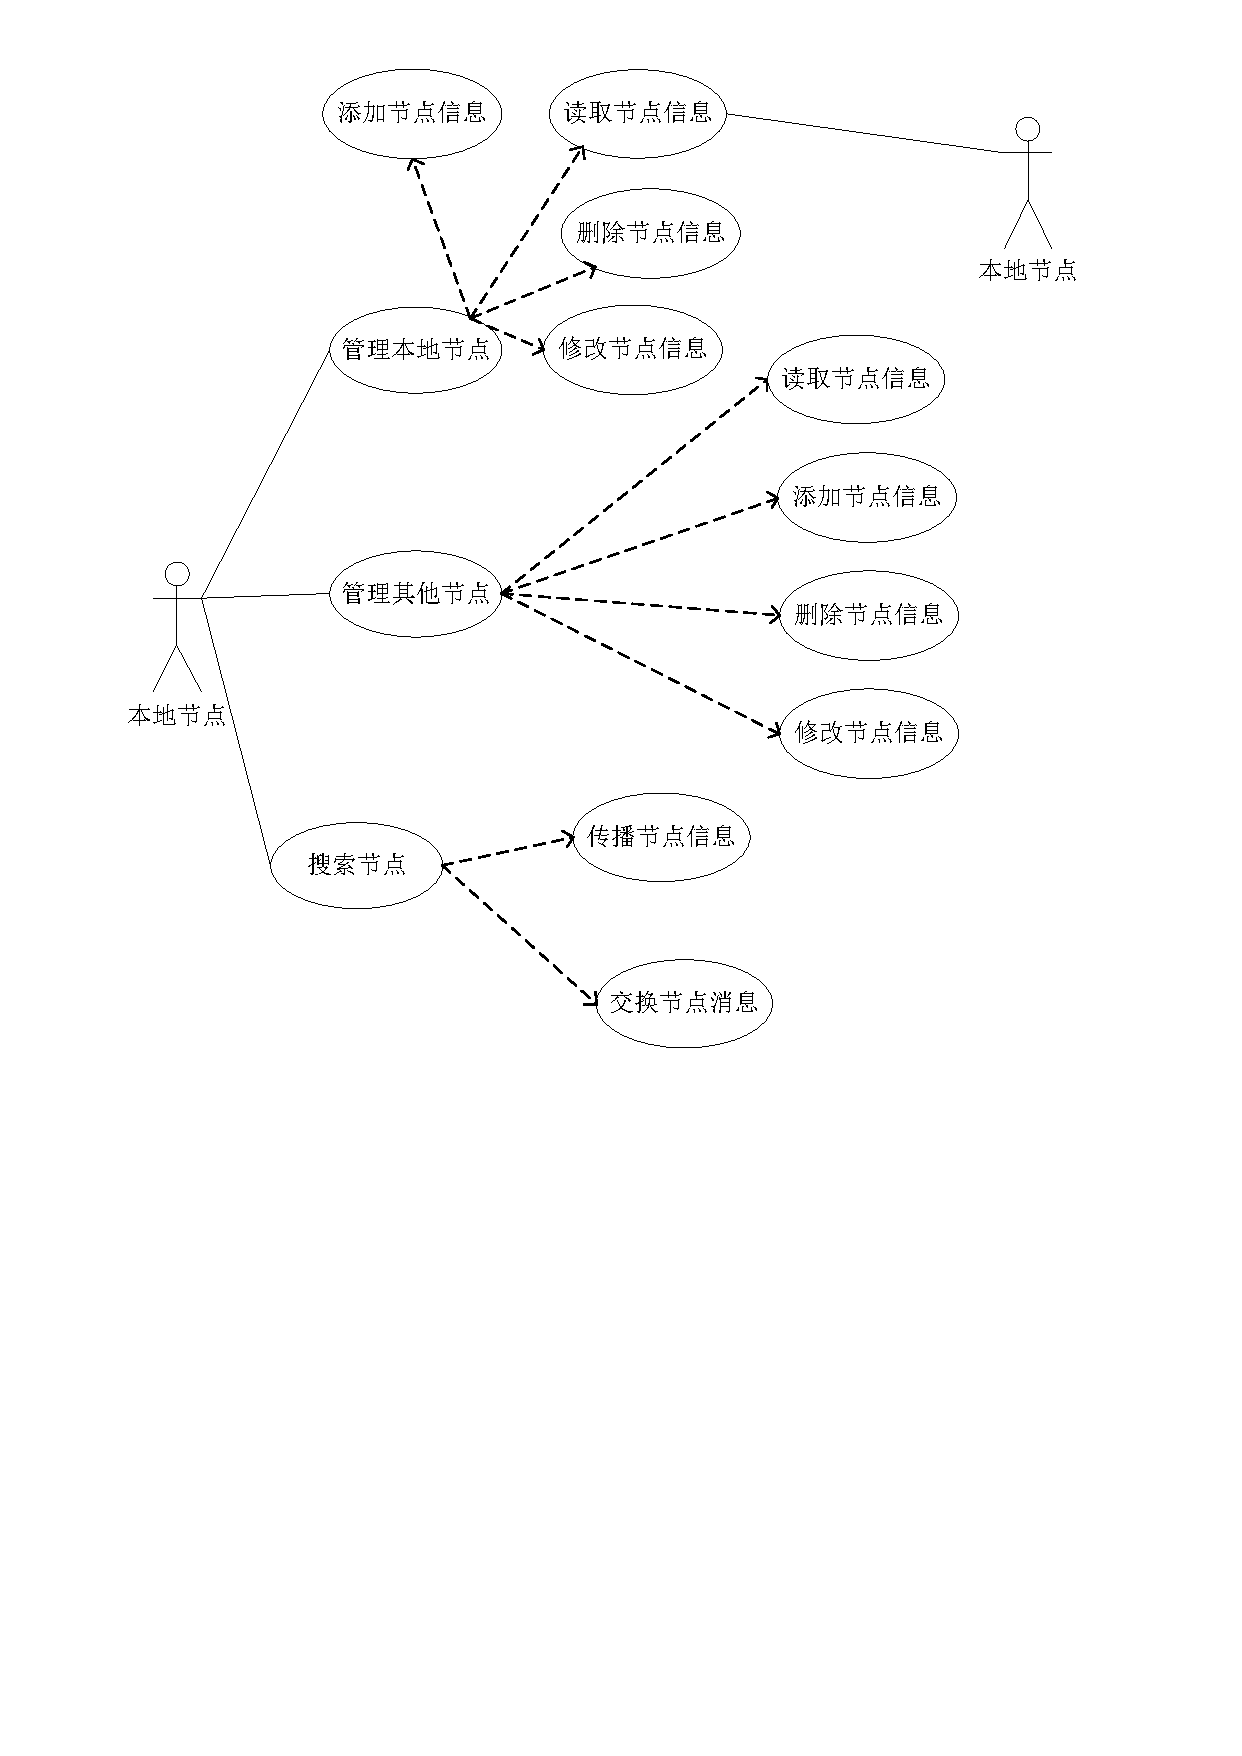
\includegraphics[width=0.9\textwidth]{usecase3.pdf}
\caption{服务端节点管理的用例图}
\label{fig:usecase3}
\end{figure}

该模块的功能主要是对本地节点和其他节点进行管理和搜索。在管理本地节点模块中,本地节点可以对本地节点的信息进行读取、添加、删除和修改,而其他节点则可以进行读取的操作。在管理其他节点模块里,只有本地节点可以对其他节点的信息进行读取、添加、删除和修改。在搜索节点模块里,本地节点可以与其他节点进行传播和交易信息。如图\ref{fig:usercase3}所示,展示了节点服务端程序中节点管理模块的用例图。

\subsubsection{服务端兴趣集管理的需求设计}
\begin{figure}[!htb]
\centering
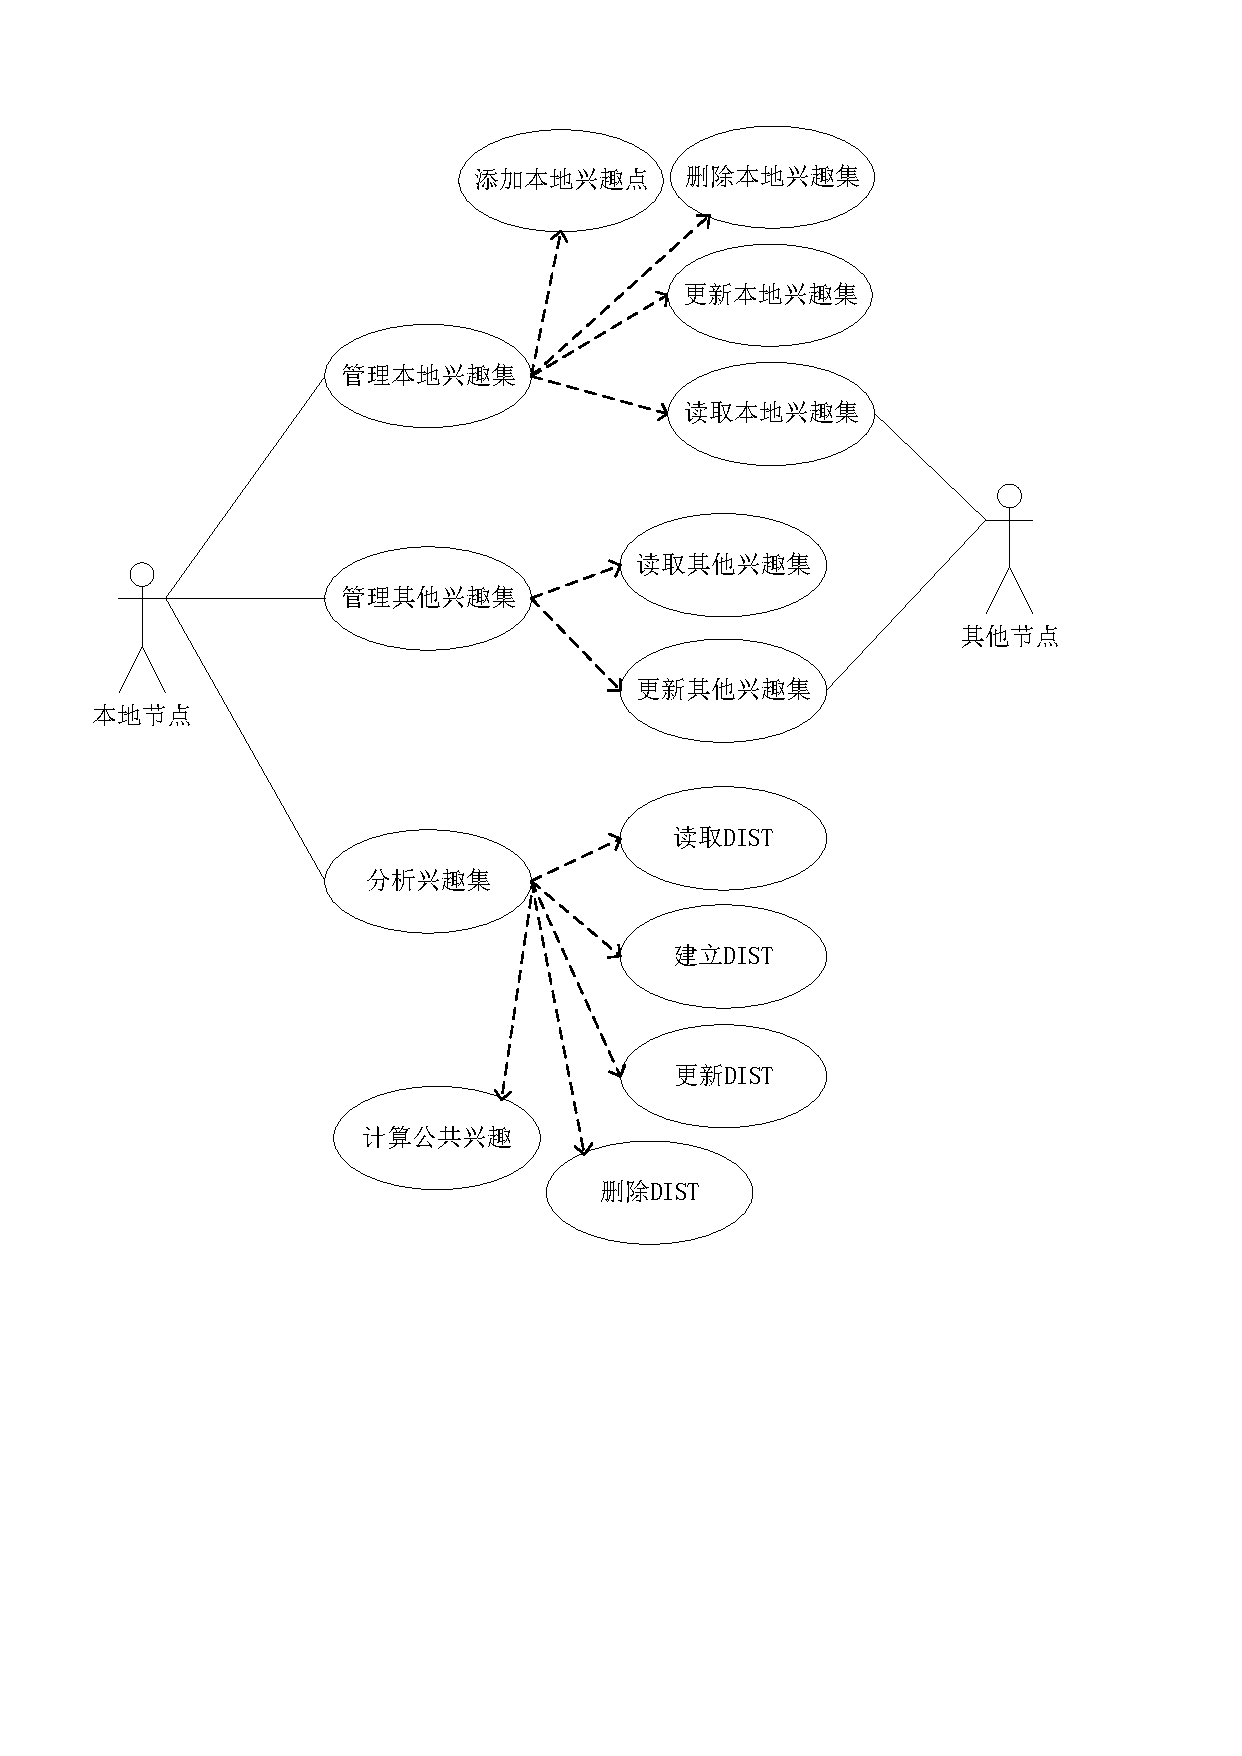
\includegraphics[width=\textwidth]{usecase4.pdf}
\caption{服务端兴趣集管理的用例图}
\label{fig:usecase4}
\end{figure}

该模块的功能主要对本地和其他的兴趣进行管理,以及对兴趣集进行分析。在管理本地兴趣集的模块里,本地节点可以对本地兴趣集进行添加、删除、更新和读取,而其他节点可以读取本地兴趣集。在管理其他兴趣集的模块中,本地节点可以对其他兴趣集进行读取和更新,其他节点则可以直接进行更新。在分析兴趣集的模块里,本地节点可以对本地存储的动态兴趣伸展树进行读取、建立、更新和删除的操作,同时也能计算给定两个兴趣集的公共兴趣。关于兴趣集的运算详情,请参见第四章的讨论。如图\ref{fig:usercase4}所示,展示了节点服务端程序中兴趣集管理模块的用例图。


\subsubsection{服务端缓存服务的需求设计}
\begin{figure}[!htb]
\centering
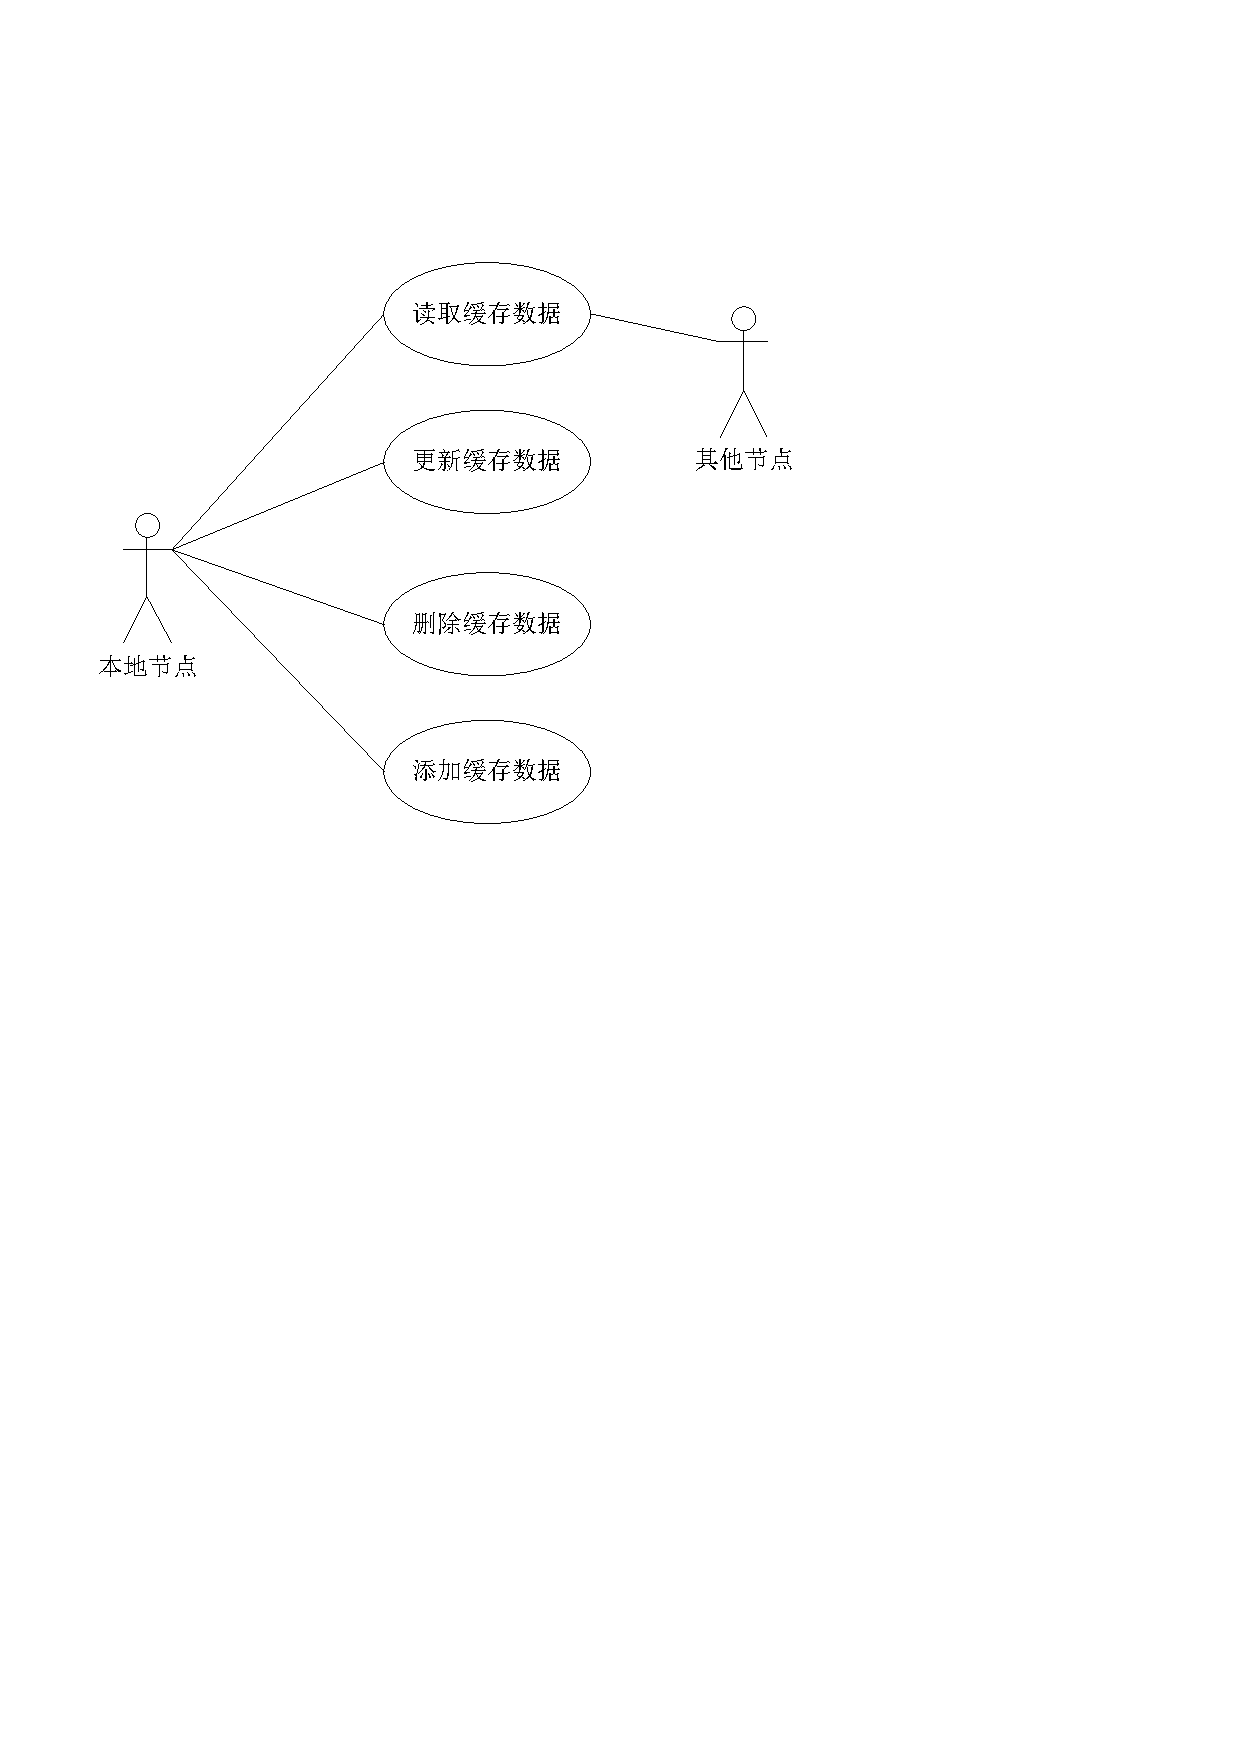
\includegraphics[width=0.6\textwidth]{usecase5.pdf}
\caption{服务端缓存管理的用例图}
\label{fig:usecase5}
\end{figure}

该模块主要提供缓存管理的功能,其中,本地节点可以对缓存中的数据进行读取、更新、删除和添加的操作,而其他节点则只能读取缓存的数据。如图\ref{fig:usercase5}所示,展示了节点服务端程序中缓存管理模块的用例图。

要注意的是,这里的缓存是为了让其他节点执行更加快速地访问,从而可以有效地减少网络带宽的占用,减少用户等待的延迟以及减少其实服务器的负载。但是缓存的大小不是无限的,特别是在用户节点上运行的机器,因此缓存的内容必须要有取舍。这里默认使用的是基于LRU(Least Recently Used)的缓存替换策略,即节点会每次替换距离上一次被访问时间最长的内容。

\subsection{主要开发技术}
节点系统主要用Java编程语言实现,辅以Python作为数据分析之用,模块间与系统间的消息传递格式为JSON,具体技术如表\ref{tbl:tech}。鉴于本系统只是一个雏形,因此使用了大量轻量级框架进行敏捷开发,在并发性等性能方面的问题暂时先不纳入考虑。

\begin{table}[ht]
\centering
\caption{原型系统开发主要技术列表}
\begin{tabular}{|c|c|} 
\hline
操作系统:& OS X 10.10.3 \\
\hline
系统后台开发语言:& JDK 1.8 \\
\hline
系统后台开发框架:& Spring、JFinal \\
\hline
后台数据库:& sqlite 3 \\
\hline
系统前端开发语言:& Html、CSS、Javascript \\
\hline
系统前端开发框架:& Bootstrap、JQuery \\
\hline
数据引擎开发语言:& Python 2.7、R \\
\hline
数据引擎计算框架:& numpy、scipy、sklearn、gensim、NLTK \\
\hline
\end{tabular}
\label{tbl:tech}
\end{table}

\subsection{节点系统的架构设计}
首先,节点系统的最大特点是既要充当服务器向外部的节点进行交互信息,也要作为客户端为本地用户提供一个可视化的浏览平台。为了满足这样的需求,节点系统的架构设计如图\ref{fig:architect}所示。

\begin{figure}[!ht]
\centering
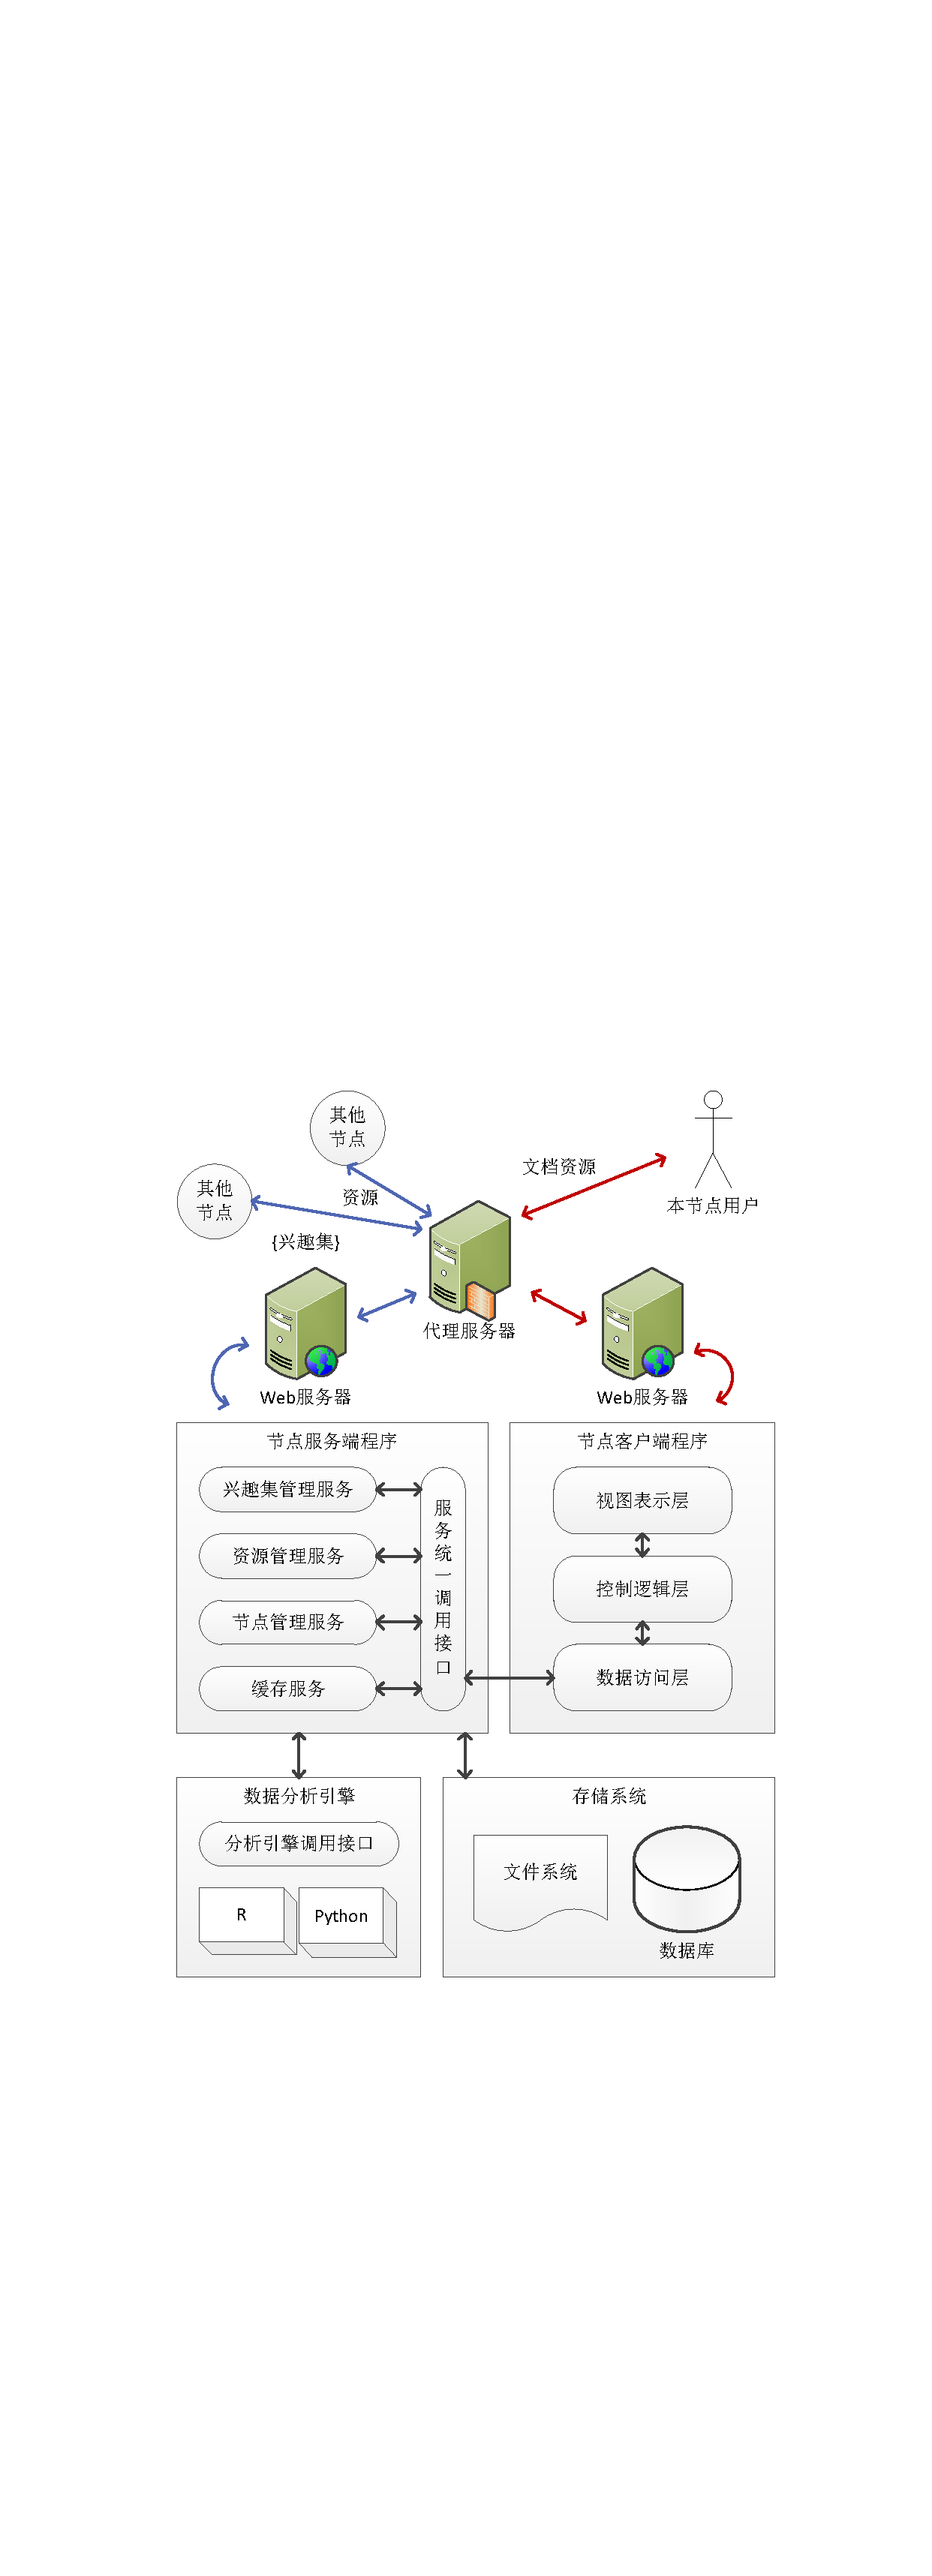
\includegraphics[width=\textwidth]{architect.pdf}
\caption{节点系统的架构示意图}
\label{fig:architect}
\end{figure}

从图中可以看到,节点系统处理的请求用户可以分为两大类:本节点的用户和其他节点的程序。其中,本节点的用户主要是对本地资源进行操作,包括发表新的文章、查看推荐的文章等。而其他节点的程序主要是与本节点交换兴趣信息和网络信息等。考虑到两种请求的独立性,我们将节点系统分为节点服务端程序和节点客户端程序两大模块,并分别运行于两个独立的web服务器中,并由代理服务器统一接受、处理并转发双方的请求。这样做的好处是模块之间保持相对地独立,作用分工明确,耦合性也比较小。

对于节点客户端程序,本质是一个运行在web服务器上的网站系统,由于其功能相对简单,主要是对资源数据的读写,因此在架构设计方面采用了如下两点方案:
\begin{itemize}
  \item MVC三层架构:在传统的J2EE架构中,控制层和业务逻辑层往往是分开的,但是文本为了快速实现原型系统,对节点客户端程序采用了更加简单的MVC架构,即将业务逻辑与页面控制合并在控制层实现。由于其功能在逻辑处理上非常简单,所以这样的实现方式并不会给系统带来多大的负担。
  \item 数据访问限制:节点客户端程序不能直接访问数据库或文件系统,而是通过节点服务端程序提供的统一接口进行操作。换句话说,整个系统对底层存储资源的调用全部集中在节点服务端程序中,这样对读写操作的隔离在设计上保证了数据的安全性,同时避免了因为多进程对数据读写导致的一致性问题。
\end{itemize}

对于节点服务端程序,其功能和模块相对复杂很多,内部主要分为四大功能模块,并且给外部暴露了一个统一的API,一方面给外来节点请求做响应,另一方面给内部节点客户端程序调用资源相关操作。在四个功能模块中,资源管理服务模块负责用户文本资源相关操作的处理,其只需对存储系统简单的读写操作。节点管理服务模块负责管理本节点的相关信息,以及在用户关注关系层和用户兴趣关系层中的节点信息,这部分对I/O的要求比较高,所以需要结合缓存服务模块一起是用。兴趣集管理服务则管理了用户兴趣模型,以及对文本进行主题分析,从而分析用户兴趣,维护了DIST、SICT等数据结构,该模块主要对文件系统有较多的读写操作,而且需要调用后台的数据分析引擎进行模型的训练和使用。缓存服务负责对节点内常用的信息进行缓存,从而增加外部节点请求的效率。

对于分析引擎来说,其目的是为了从用户的行为和文本中挖掘出用户的兴趣,并给兴趣集管理模块提供支持。该分析引擎提供了一个统一调用的接口,用于封装后台异构的数据分析模块,比如R和Python,当然还可以集成更多其他的分析引擎。

对于存储系统来说,这里用到了关系型数据库和文件系统。数据库主要存储结构化的信息,从而方便快速索引,而文件系统则存储文本资源、缓存等。

\subsection{节点系统的存储机制}
本系统共有三种存储的方式,即数据库、文件系统和内存,下面将具体讨论三种类型的存储介质所保存的数据。

\subsubsection{节点系统的数据库}
数据库中主要存储的是结构化数据,从而便于快速查找。下面的这些数据是存在数据库中。
\begin{enumerate}
\item nodes表 \\
该表用于存储P2P网络上除本节点之外的其他节点的基本信息,表的结构如下所示。
\begin{table}[!htb]
  \centering
  \begin{tabular}{|l|l|l|}
    \hline
    属性 & 类型 & 说明 \\
    \hline
    id & integer & PK.节点编号 \\
    \hline
    ipv4 & varchar(32) & 节点的IPv4地址 \\
    \hline
    ipv6 & varchar(128) & 节点的IPv6地址 \\
    \hline
    port & integer & 节点可供访问的端口 \\
    \hline
    mac & varchar(128) & 节点的物理MAC地址\\
    \hline
    bandwidth & double & 节点所处位置的平均带宽 \\
    \hline
    longtitude & varchar(32) & 物理位置的经度 \\
    \hline
    latitude & varchar(32) & 物理位置的纬度 \\
    \hline
  \end{tabular}
\end{table}
\item interest\_sets表 \\
该表用于存储在用户兴趣关系层中节点的兴趣集或者兴趣导向边的兴趣集,表中的每一条记录表示一个用户兴趣元。表的结构如下所示。
\begin{table}[!htb]
  \centering
  \begin{tabular}{|l|l|l|}
    \hline
    属性 & 类型 & 说明 \\
    \hline
    id & integer & PK. \\
    \hline
    node\_id & integer & FK.节点编号 \\
    \hline
    type & varchar(32) & 兴趣元的类型:节点或兴趣导向边 \\
    \hline
    interest\_id & integer & 全局兴趣点的编号 \\
    \hline
    weight & double & 该兴趣点的权重 \\
    \hline
  \end{tabular}
\end{table}
\item resources表 \\
该表用于存储用户发表的或者接受的文本资源,表的结构如下所示。
\\ \\
\begin{table}[!htb]
  \centering
  \begin{tabular}{|l|l|l|}
    \hline
    属性 & 类型 & 说明 \\
    \hline
    id & integer & PK.文本资源编号 \\
    \hline
    node\_id & integer & FK.发布资源的节点编号 \\
    \hline
    topics & text & 文本资源的主题向量 \\
    \hline
    created & datetime & 资源创建时间 \\
    \hline
    modified & datetime & 资源修改时间 \\
    \hline
  \end{tabular}
\end{table}
\item reviews表 \\
该表用于存储用户对文本资源的反馈,表的结构如下所示:
\begin{table}[!htb]
  \centering
  \begin{tabular}{|l|l|l|}
    \hline
    属性 & 类型 & 说明 \\
    \hline
    id & integer & PK.资源反馈的编号 \\
    \hline
    resource\_id & integer & FK.资源的编号 \\
    \hline
    node\_id & integer & FK.用户反馈所在的节点编号 \\
    \hline
    duration & double & 查看资源的时间 \\
    \hline
    comment & varchar(1024) & 评论内容 \\
    \hline
    created & datetime & 反馈创建的时间 \\
    \hline
  \end{tabular}
\end{table}
\end{enumerate}

\subsubsection{节点系统的文件系统}
在文件系统中主要存储一些在关系型数据库中无法存储的非结构化的数据,主要包括以下几种类型:
\begin{itemize}
  \item 文本资源:
    由于纯文本的资源文件大小浮动很大,是典型的非结构化数据,如果在数据库中作为text类型进行存储往往会影响到查询性能。而且对于互联网资源中的文本来说,往往使用html语言来描述的,还会包括图片、超链接、字体格式等内容。对于这种情况,本系统将所有的资源均存储在文件系统中。
  \item 全局主题:在第三章和第四章对文章的主题进行了定义,考虑到主题是一个关于词汇的向量,维度十分巨大,因此在数据库中很难用这么多行列来存储。因此这里的做法是将主题向量表示成JSON的格式,从而方便各种编程语言调用。
  \item 兴趣树:兴趣树分为DIST和SICT。其中,DIST的特征是动态变化十分频繁,但是结构不是很大,所以这里只是在文件系统上存储一个序列化的数据结构文件,当系统运行时,会自动将该数据结构反序列化载入内存,从而加快处理速度,当系统要关闭时,会向文件系统重新更兴趣树文件。SICT的特征则相反,其一般是静态保持不变的,但结构十分庞大,因此系统将这个结构依然存储为文件,但是载入内存是选择局部载入,这样节省了内存的开销。
  \item 词汇表:词汇表相当于电子词典,有两种存储方式。第一,可以建立带有索引的词汇表文件,这样管理的代价比较大,但是处理速度很快;第二,直接调用公开的API,英文词库如WordNet\footnote{http://wordnet.princeton.edu/}等,但是在网络开销上会有一定的影响。
\end{itemize}

\subsubsection{节点系统的内存}
将数据存储在内存中是为了提高系统的处理速度,除了上述提到的需要序列化的数据结构之外,缓存和路由表是内存中最重要的内容。与传统的RAM一样,这里的缓存数据会在系统断电后直接消失,因此,为了解决这个问题,我们采用了定期备份重要数据至文件系统的策略。所谓重要的信息,一般是指访问次数相对较多的其他节点列表、请求次数较多的文本资源等等。

\subsection{节点系统的关键功能实现}
//TODO

\subsection{小结}
本章主要说明了基于P2P网络的信息自主流动机制的原型系统。首先分析了不同角色之间拥有的功能有哪些,并用用例图详细分析了各个模块的功能需求。然后,为了使得系统能够同时充当服务器和客户端,文中提出了一种全新的系统架构,将节点服务端程序和节点客户端程序分为两个web应用,并使得两者分别向外提供不同的调用接口,供本地用户或者外来节点使用。此外,本章还说明了系统在存储方面的实现细节,采用了三种存储介质:数据库、文件系统和内存,分别为了适应不同类型的数据和资源。
